% (c) 2012 Claudio Carboncini - claudio.carboncini@gmail.com
% (c) 2012 Dimitrios Vrettos - d.vrettos@gmail.com
\chapter{Espressioni letterali e valori numerici}
\section{Lettere}
\subsection{Lettere per esprimere formule}
\begin{exrig}
 \begin{esempio}
 In tutte le villette a schiera di recente costruzione del nuovo quartiere Stella, vi è un
terreno rettangolare di larghezza~$12\unit{m}$ e lunghezza~$25\unit{m}$. Quanto misura la superficie del terreno?
\begin{center}
 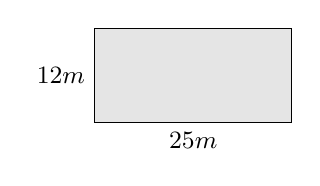
\begin{tikzpicture}[x=5mm, y=5mm,font=\small]
\definecolor{area}{gray}{0.9}
\draw [fill=area] (0,0) rectangle (5,2.4); 

\node[below] at (2.5,0) {$25\unit{m}$};
\node [left] at (0,1.2) {$12\unit{m}$};

\end{tikzpicture}
\end{center}

Il prodotto delle dimensioni rappresenta la misura richiesta:~$S=(25\cdot 12)\unit{m}^{2}=300\unit{m}^2$.
 \end{esempio}
\end{exrig}

Il semplice problema che abbiamo risolto è relativo ad un caso particolare; quel terreno con
quelle dimensioni. Ma se le dimensioni fossero diverse?

La procedura per determinare la misura della superficie ovviamente è sempre la stessa e la possiamo esprimere con la
formula~$A=b\cdot h$ nella quale abbiamo indicato con~$b$ la misura di una dimensione (base) e con~$h$ la misura dell'altra
dimensione (altezza), assegnate rispetto alla stessa unità di misura.

\osservazione La formula ha carattere generale e serve ogniqualvolta si chiede di determinare la superficie di un rettangolo,
note le misure delle dimensioni (base e altezza) rispetto alla stessa unità di misura.

In geometria si utilizzano tantissime formule che ci permettono di esprimere perimetro e
area delle figure piane, superficie laterale e totale e volume dei solidi. Nelle formule le lettere sostituiscono le
misure di determinate grandezze, tipiche di quella figura o di quel solido.

\ovalbox{\risolvi \ref{ese:9.1}}

\subsection{Lettere per descrivere schemi di calcolo}
\begin{exrig}
 \begin{esempio}
 L'insegnante chiede agli alunni di scrivere <<il doppio della somma di due numeri>>.

\begin{itemize*}
\item Antonella scrive:~$2\cdot (3+78)$;
\item Maria chiede <<Quali sono i numeri? Se non li conosco non posso soddisfare la richiesta>>;
\item Giulia scrive:~$2\cdot (a+b)$.
\end{itemize*}
Maria si è posta il problema ma non ha saputo generalizzare la richiesta. Antonella si è limitata ad un caso
particolare. Giulia ha espresso con una formula l'operazione richiesta dall'insegnante.
 \end{esempio}
\end{exrig}

\osservazione L'uso di lettere dell'alfabeto per indicare numeri ci permette di generalizzare uno schema di calcolo, cioè ci consente di scrivere un algoritmo.

\begin{definizione}
 Un'\emph{espressione letterale} o \emph{espressione algebrica} è uno schema di calcolo in cui compaiono numeri e lettere
legati dai simboli delle operazioni.
\end{definizione}

Per scrivere un'espressione letterale ci si deve attenere a regole precise, quelle stesse che utilizziamo per scrivere
espressioni numeriche.

Per esempio, la scrittura~``$3\cdot 4+$'' non è corretta, in quanto il simbolo~``$+$'' dell'addizione deve essere seguito da un
altro numero per completare l'operazione. Analogamente non è corretta l'espressione letterale~``$a\cdot c+$''.

Come nelle espressioni numeriche, anche nelle espressioni letterali le parentesi indicano la priorità di alcune operazioni rispetto ad altre.
La formula~$a\cdot (x+y)$ specifica ``il prodotto di un numero per la somma di altri due''. Essa è diversa da  $a\cdot x+y$
che rappresenta ``il prodotto di due numeri sommato a un terzo numero''.

\vspazio\ovalbox{\risolvii \ref{ese:9.2}, \ref{ese:9.3}}

\subsection{Lettere per esprimere proprietà}

Le proprietà delle operazioni tra numeri si esprimono con lettere per indicare che valgono per numeri
qualsiasi.
La scrittura ``$(a+b)+c=a+(b+c)$'', per esempio, esprime la proprietà associativa dell'addizione. In essa le lettere~$a$, $b$ e $c$ indicano
numeri qualsiasi. I due schemi di calcolo ci dicono che per sommare tre numeri è indifferente aggiungere alla somma
dei primi due il terzo oppure aggiungere al primo la somma degli altri due.

\vspazio\ovalbox{\risolvii \ref{ese:9.4}, \ref{ese:9.5}, \ref{ese:9.6}, \ref{ese:9.7}, \ref{ese:9.8}, \ref{ese:9.9}, \ref{ese:9.10}, \ref{ese:9.11}}

\section{Il valore numerico di un'espressione letterale}

Ogni espressione letterale rappresenta uno schema di calcolo in cui le lettere che vi compaiono sostituiscono numeri.
L'espressione letterale

\[2\cdot x^{2}+x\]

\noindent traduce una catena di istruzioni che in linguaggio naturale sono così
descritte: ``prendi un numero ($x$); fanne il quadrato ($x^2$); raddoppia quanto ottenuto ($2\cdot x^2$); aggiungi al risultato il numero preso inizialmente ($2\cdot x^{2}+x$)''.

Questa catena di istruzioni si può anche rappresentare in modo schematico
\[x\quad\rightarrow\quad x^{2}\quad\rightarrow\quad~2\cdot x^{2}\quad\rightarrow\quad~2\cdot x^{2}+x\]
e può essere usata per istruire un esecutore a ``calcolare'' l'espressione letterale
quando al posto della lettera~$x$ si sostituisce un numero.

Calcoliamo il valore dell'espressione~$2\cdot x^{2}+x$, sostituendo alla lettera $x$ il numero naturale~5.
Seguiamo la schematizzazione~$x\rightarrow x^{2}\rightarrow~2\cdot x^{2}\rightarrow~2\cdot x^{2}+x$ e otteniamo:
$5\rightarrow~25\rightarrow~50\rightarrow~55$.
Il risultato è~$55$.
Più brevemente scriviamo~$5$ nell'espressione letterale al posto di~$x$: otteniamo l'espressione numerica~$2\cdot 5^{2}+5$
il cui risultato è~$55$.

E se al posto di~$x$ sostituiamo~$-5$? Otteniamo un risultato diverso? Eseguiamo la sostituzione di $x$ con $-5$ e abbiamo: $2\cdot (-5)^{2}+(-5)=\ldots$ Lasciamo a te il calcolo finale. Ti sarai accorto che il
risultato è cambiato.

 \begin{definizione}
In un'espressione letterale le \emph{lettere} rappresentano le \emph{variabili} che assumono specifiche quantità
quando vengono sostituite da numeri.
Chiamiamo \emph{valore} di un'espressione letterale il risultato numerico che si ottiene eseguendo le operazioni indicate dallo
schema di calcolo quando alle lettere sostituiamo un determinato numero. Il valore di un'espressione letterale dipende dal \emph{valore assegnato} alle sue variabili.
\end{definizione}

D'ora in poi quando scriveremo un'espressione letterale in cui compare
l'operazione di moltiplicazione, tralasceremo il puntino fin qui usato per evidenziare l'operazione.
Così l'espressione~$5\cdot a^{2}+\dfrac{3}{8}\cdot a\cdot b-7\cdot b^{2}$ verrà scritta in modo
più compatto~$5a^{2}+\dfrac{3}{8}ab-7b^{2}$.

\begin{exrig}
 \begin{esempio}
Calcolare il valore numerico della seguente espressione:~$3a(a-b)$ per~$a=1$, $b=1$.

\emph{Svolgimento}:~$3\cdot 1\cdot (1-1)=3\cdot 1\cdot 0=0$.
\end{esempio}
 \end{exrig}

\ovalbox{\risolvii \ref{ese:9.12}, \ref{ese:9.13}, \ref{ese:9.14}, \ref{ese:9.15}, \ref{ese:9.16}, \ref{ese:9.17}, \ref{ese:9.18}, \ref{ese:9.19}, \ref{ese:9.20}, \ref{ese:9.21}, \ref{ese:9.22}}

\section{Condizione di esistenza di un'espressione letterale}
Ti proponiamo adesso alcuni casi particolari per
l'espressione~$E=\dfrac{x-y}{3x}$.

\paragraph{Caso I:} $x=1\,\wedge\, y=1\, \Rightarrow\, E=0$.
%
%\begin{center}
%\begin{tabular*}{.2\textwidth}{@{\extracolsep{\fill}}*{3}{c}}
%\toprule
%$x$ & $y$ & $E$\\
%1 & 1 & 0\\
%\bottomrule
%\end{tabular*}
%\end{center}

Il numeratore della frazione è~0, mentre il denominatore vale~3; il
calcolo finale è dunque~$\frac{0}{3}=0$.
Vi sono, secondo te, altre coppie di valori $(x;y)$ che fanno
assumere ad~$E$ quello stesso valore?

\paragraph{Caso II:} $x=0\,\wedge\, y=25\, \Rightarrow\, E=?$.
%\begin{center}
%\begin{tabular*}{.2\textwidth}{@{\extracolsep{\fill}}*{3}{c}}
%\toprule
%$x$ &$y$ &$E$\\
%0 &25 &?\\
%\bottomrule
%\end{tabular*}
%\end{center}

Invece di mettere un valore ad~$E$, abbiamo messo punto di domanda
perché in questo caso il numeratore della frazione è~$-25$ mentre
il denominatore vale~0; il calcolo finale è dunque~$-{\frac{25}{0}}$, impossibile.
Vi sono, secondo te, altre coppie di valori $(x;y)$ che rendono
impossibile il calcolo del valore per~$E$?

Non possiamo allora concludere che per ogni coppia di numeri razionali~$(x;y)$ 
l'espressione~$E$ assume un numero razionale.
Per poter calcolare il valore di~$E$ non possiamo scegliere coppie aventi~$x$ 
uguale a zero.
Scriveremo quindi come premessa alla ricerca dei valori di~$E$ la \emph{Condizione di Esistenza} ($\CE$)~$x\neq~0$.

L'esempio appena svolto ci fa capire che di fronte a
un'espressione letterale dobbiamo riflettere sullo
schema di calcolo che essa rappresenta prima di assegnare valori alle
variabili che vi compaiono.

Se l'espressione letterale presenta una divisione in cui
il divisore contiene variabili, dobbiamo stabilire la~$\CE$, 
eliminando quei valori che rendono nullo il divisore.
Per comprendere la necessità di porre le condizioni
d'esistenza ricordiamo la definizione di divisione.

Quanto fa~15 diviso~5? In forma matematica:~$15:5=3$ perché $3\cdot 5=15$. Quindi, 
generalizzando~$a:b=c$ se~$c\cdot b=a$.

Vediamo ora cosa succede quando uno dei numeri è~0:

\begin{itemize*}
 \item quanto fa~$0:5$? Devo cercare un numero che moltiplicato per~5 mi dia~0: trovo solo~0; infatti~$0\cdot 5=0$.
 \item quanto fa~$15:0$? Devo cercare un numero che moltiplicato per~0 mi dia~15:
non lo trovo; infatti nessun numero moltiplicato per~0 fa~15. Quindi,
$15:0$ è impossibile perché non esiste alcun
$x$ per il quale~$x\cdot 0=15$.
 \item quanto fa~$0:0$? Devo cercare un numero che moltiplicato per~0 mi dia~0:
non ne trovo solo uno. Infatti, qualunque numero moltiplicato per~0
fa~0. Per esempio, $0:0=33$; infatti
$33\cdot 0=0$. Ma anche~$0:0=\np{-189,6}$;
infatti~$\np{-189,6}\cdot 0=0$. E anche $0:0=0$;
infatti~$0\cdot 0=0$. 
Ancora~$0:0=10^{99}$, infatti~$10^{99}\cdot 0=0$.
Quindi~$0:0$ è indeterminato perché
non è possibile determinare un unico~$x$ tale che~$x\cdot 0=0$,
ma per qualunque valore di~$x$ si ha~$x\cdot 0=0$.
\end{itemize*}

Consideriamo l'espressione letterale~$E=\dfrac{a-b}{a+b}$ dove~$a$ e~$b$ 
rappresentano numeri razionali.
Premettiamo:

\begin{enumeratea}
 \item la descrizione a parole dello schema di calcolo:
``divisione tra la differenza di due numeri e la loro
somma'';
 \item la domanda che riguarda il denominatore: ``quand'è che la somma di
due numeri razionali dà come rislutato~0?'';
 \item la~$\CE$: ``$a$ e~$b$ non devono essere numeri opposti''.
\end{enumeratea}

Siamo ora in grado di completare la tabella:
\begin{center}
\begin{tabular*}{.8\textwidth}{l@{\extracolsep{\fill}}*{5}{c}}
\toprule
$a$ & 3 &0 & $\frac{3}{4}$ &$-{\frac{5}{8}}$ & $-{\frac{19}{2}}$ \\
$b$ & $-3$ & $-{\frac{1}{2}}$ & 0 &$\frac{5}{8}$ & $-{\frac{19}{2}}$ \\
\midrule
$E=\frac{a-b}{a+b}$ & & & & &\\
\bottomrule
\end{tabular*}
\end{center}

Dalla~$\CE$, ci accorgiamo subito che la
prima coppia e la quarta sono formate da numeri opposti, pertanto non
possiamo calcolare il valore di~$E$ ad esse relativo. L'ultima
coppia è formata da numeri uguali pertanto la loro differenza è~0, così
il numeratore si annulla e quindi il valore di~$E$ è~0. 
Per la coppia~$\left(0;-\frac{1}{2}\right)$ il valore di~$E$ è~$-1$ mentre è~1 per
la coppia~$\left(\frac{3}{4};0\right)$.
La tabella verrà quindi così completata:

\begin{center}
\begin{tabular*}{.8\textwidth}{l@{\extracolsep{\fill}}*{5}{c}}
\toprule
$a$ & 3 &0 & $\frac{3}{4}$ &$-{\frac{5}{8}}$ & $-{\frac{19}{2}}$ \\
$b$ & $-3$ & $-{\frac{1}{2}}$ & 0 &$\frac{5}{8}$ & $-{\frac{19}{2}}$ \\
\midrule
$E=\frac{a-b}{a+b}$ &impossibile & $-1$& 1& impossibile&0\\
\bottomrule
\end{tabular*}
\end{center}

Cosa succede per la coppia~$(0;0)$?

\vspazio\ovalbox{\risolvi \ref{ese:9.24}}
\newpage

 % (c) 2012 -2014 Claudio Carboncini - claudio.carboncini@gmail.com
% (c) 2012 -2014 Dimitrios Vrettos - d.vrettos@gmail.com
\section{Esercizi}
\subsection{Esercizi dei singoli paragrafi}
\subsubsection*{9.1 - Espressioni letterali e valori numerici}

\begin{multicols}{2}
\begin{esercizio}[\Ast]
\label{ese:9.1}
Esprimi con una formula l'area della superficie della zona colorata della figura qui a fianco, %\ref{fig:9.1},
indicando con~$l$ la misura del lato~$AB$ del quadrato grande e
con~$b$ la misura di~$AC$ del quadrato piccolo.
%
%\emph{Svolgimento}: l'area del quadrato è \ldots,
%l'area di ciascuno dei quadratini bianchi è \ldots\, Pertanto l'area della
%superficie in
%grigio è \ldots
\begin{center}
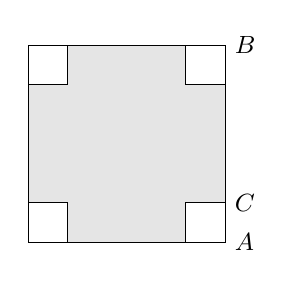
\begin{tikzpicture}[x=5mm, y=5mm,font=\small]
\definecolor{area}{gray}{0.9}
\draw [fill=area] (0,0) rectangle (5,5); 
\foreach \x in {0,4}{
\draw[fill=white] (\x,0) rectangle (\x+1,1);
\draw[fill=white] (\x,4) rectangle (\x+1,5);}
\node[right] at (5,0) {$A$};
\node [right] at (5,5) {$B$};
\node [right] at (5,1) {$C$};
\end{tikzpicture}
\end{center}
\end{esercizio}
\end{multicols}

\begin{esercizio}[\Ast]
\label{ese:9.2}
Scrivi l'espressione algebrica letterale relativa alla frase ``eleva al quadrato la differenza tra il cubo di un
numero e il doppio del suo quadrato''.

\emph{Svolgimento}: detto~$a$ il numero generico, il cubo di~$a$ si indica con \ldots,
il doppio del quadrato di~$a$ si indica con \ldots e infine
il quadrato della differenza sarà: \ldots
\end{esercizio}

\begin{esercizio}
\label{ese:9.3}
Traduci in parole della lingua italiana il seguente schema di calcolo:~$(a-b)^{3}$

\emph{Svolgimento}: ``Eleva al \ldots\ldots la differenza tra \ldots\ldots''
\end{esercizio}

%\begin{esercizio}
% \label{ese:9.4}
%Individua tra le espressioni letterali sottostanti, quelle scritte correttamente:
%\begin{enumeratea}
%\spazielenx
% \item $b\cdot {\frac{4}{5}}+\left(3-\frac{7}{2}\right)\cdot a-a$;
% \item $a\cdot 2-b^{4}$;
% \item $x\cdot (a-b)^{2}+(x-3)$;
% \item $x^{y}-a:2$;
% \item $-a+4b+c$;
% \item $\frac{a\cdot 1}{2}-\frac{a}{2}$.
%\end{enumeratea}
%\end{esercizio}
%\end{multicols}

\begin{esercizio}
\label{ese:9.4} %ex9.5
 Collega con una freccia la proprietà dell'operazione con la sua scrittura attraverso lettere:
 \begin{multicols}{2}
 \noindent
 Commutativa dell'addizione\\
 Associativa della moltiplicazione\\
 Distributiva prodotto rispetto alla somma\\
 $a\cdot (x+y)=a\cdot x+a\cdot y$\\
 $\left(a\cdot b\right)\cdot c=a\cdot \left(b\cdot c\right)$\\
 ${a+b=b+a}$
 \end{multicols}
\end{esercizio}

%\begin{esercizio}
%\label{ese:9.6}
%Esprimere con le lettere la proprietà commutativa della moltiplicazione
%
%\emph{Svolgimento}: ``considerati~$a$ e~$b$ due numeri qualsiasi, la proprietà commutativa si esprime per mezzo dell'espressione \ldots\ldots; cioè \ldots\ldots\ldots''
%\end{esercizio}

%\begin{multicols}{2}
\begin{esercizio}
\label{ese:9.5} %{ese:9.7}
Scrivi la formula che ci permette di calcolare l'area di un trapezio avente base maggiore~$B=5\unit{cm}$, base minore~$b=2\unit{cm}$ e altezza~$h=4\unit{cm}$.
\end{esercizio}

\begin{esercizio}[\Ast]
\label{ese:9.6} %{ese:9.8}
Scrivi la formula che ci consente di calcolare perimetro e area di un quadrato il cui lato misura~$2x$.
\end{esercizio}

\begin{esercizio}
\label{ese:9.7} %{ese:9.9}
Determina l'altezza~$h$ relativa all'ipotenusa~$BC$ del triangolo rettangolo~$ABC$.

Caso \emph{numerico}:~$\overline{AB}=8\unit{m}$, $\overline{AC}=15\unit{m}.$

Caso \emph{generale}: Indica con~$x$ e~$y$ le misure dei cateti, e determina la formula per calcolare la misura di~$h$.
\end{esercizio}

\begin{esercizio}
\label{ese:9.8} %{ese:9.10}
\begin{multicols}{2}
Il volume della scatola della figura %~\ref{fig:9.2} 
avente le dimensioni di~$7\unit{cm}$, $10\unit{cm}$, $2\unit{cm}$ è~$\ldots$

Generalizza la questione indicando con~$a$, $b$, $c$ le misure delle sue dimensioni \ldots

Se raddoppiamo ciascuna dimensione allora il volume diventa
% \begin{enumeratea}

 A)~$2abc$;

 B)~$a^{2}b^{2}c^{2}$;

 C)~$6abc$;

 D)~$8abc$.
% \end{enumeratea}
\begin{center}
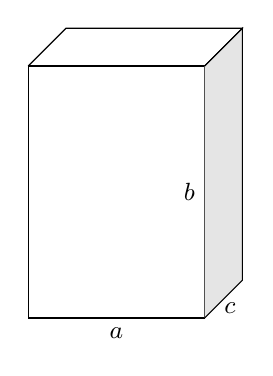
\begin{tikzpicture}[x=4mm, y=4mm,font=\small,scale=.8]
\definecolor{area}{gray}{0.9}
\draw(0,0) rectangle (7,10); 
\draw[fill=area, draw=black](7,0) -- (8.5,1.5)-- (8.5,11.5)--(7,10);
\draw(0,10) -- (1.5,11.5)-- (8.5,11.5)--(7,10);

\node[below] at (3.5,0) {$a$};
\node[left] at (7,5) {$b$};
\node[below] at (8,1) {$c$};
\end{tikzpicture}
\end{center}
\end{multicols}
\end{esercizio}

\begin{esercizio}[\Ast]
\label{ese:9.9} %{ese:9.11}
Scrivi sotto forma di espressioni letterali le seguenti frasi:
 \begin{enumeratea}
 \item moltiplica~$a$ per l'inverso di~$a$;
 \item sottrai ad~$a$ l'inverso di~$b$;
 \item sottrai il doppio di~$a$ al cubo di~$a$.
 \item moltiplica~$a$ per l'opposto del cubo di~$a$:
 \item somma al triplo di~$a$ il doppio del quadrato di~$b$;
 \item moltiplica l'inverso di~$b$ per il quadrato dell'inverso di~$a$;
 \end{enumeratea}
\end{esercizio}

\begin{esercizio}[\Ast]
\label{ese:9.10} %{ese:9.12}
Scrivi sotto forma di espressioni letterali le seguenti frasi:
 \begin{enumeratea}
 \item somma al cubo di~$a$ il quadrato della somma di~$a$ e~$b$;
 \item dividi il quadrato di~$a$ per il triplo del cubo di~$b$;
 \item moltiplica il quadrato di~$b$ per l'inverso del cubo di~$a$;
 \item il cubo di un numero, aumentato di~2, è uguale al quadrato della differenza tra lo stesso numero e uno;
 \item il reciproco della somma dei quadrati di~$a$ e di~$b$;
 \item il cubo della differenza tra~1 e il cubo di~$a$;
 \item la somma dei quadrati di~$a$ e di~$b$ per il quadrato della differenza tra~$a$ e~$b$.
 \end{enumeratea}
\end{esercizio}
%\end{multicols}

\begin{esercizio}[\Ast]
\label{ese:9.11} %{ese:9.17}
Scrivi con una frase le seguenti espressioni
\begin{multicols}{3}
 \begin{enumeratea}
 \item $3a$;
 \item $\dfrac{2a}{3b^{2}}$.
 \item $2b-5a$;
 \item $a {\dfrac{1}{a}}$;
 \item $(a+b)^{2}$;
 \item $\dfrac{3x+y}{2x^{2}}$.
 \end{enumeratea}
\end{multicols}
\end{esercizio}

%\begin{esercizio}
%\label{ese:9.18}
%Scrivi con una frase le seguenti espressioni
%\begin{multicols}{4}
% \begin{enumeratea}
%\spazielenx
% \item $2b-5a$;
% \item $a {\dfrac{1}{a}}$;
% \item $(a+b)^{2}$;
% \item $\dfrac{3x+y}{2x^{2}}$.
% \end{enumeratea}
%\end{multicols}
%\end{esercizio}

\subsubsection*{9.2 - Il valore numerico di un'espressione letterale}

\begin{esercizio}
\label{ese:9.12} %{ese:9.13}
Consideriamo l'espressione letterale~$E=-3a+2(-a+1)$.

Osserviamo che vi compare una sola variabile, la lettera~$a$; supponiamo che~$E$ rappresenti uno schema di calcolo tra
numeri interi relativi. Determiniamo il valore dell'espressione per alcuni valori della variabile:
\begin{align*}
a =-2 & \quad\Rightarrow\quad E =-3\cdot (-2)+2\cdot (-(-2)+1) =6+2\cdot (2+1) =6+6 =12 \\
a =+1 & \quad\Rightarrow\quad E =-3\cdot (1)+2\cdot(-(1)+1) =-3+2\cdot (-1+1) =-3+0 =-3 \\
a =-1 & \quad\Rightarrow\quad E =-3\cdot (\ldots)+2\cdot (\ldots +1) =\ldots \ldots \ldots
\end{align*}

Completa la seguente tabella.

 \begin{tabular*}{.9\textwidth}{@{\extracolsep{\fill}}*{9}{c}}
 \toprule
 $a$ & $-2$ & $1$ & $-1$ & $0,1$ & $\dfrac{4}{5}$ & $-\dfrac{7}{5}$ & $-11$ &$0$\vspace{1.05ex}\\
 \midrule
 $E=-3a+2(-a+1)$& $12$ & $-3$ &	& & & & &\\
 \bottomrule
 \end{tabular*}
\end{esercizio}

\begin{esercizio}[\Ast]
\label{ese:9.13} %{ese:9.15}
Calcolare il valore numerico dell'espressione:~$\dfrac{a}{a-3}+\dfrac{b}{3-b}$ per~$a = -1$, $b = 0$.

\emph{Svolgimento}:~$\dfrac{-1}{-1-3}+\dfrac{0}{3-0}= \ldots\ldots$
\end{esercizio}
\pagebreak
\begin{esercizio}[\Ast]
\label{ese:9.14} %{ese:9.14}
Calcola il valore dell'espressione letterale $E=\dfrac{3}{7}ab-\dfrac{1}{2}(a-b)+a-b$ le cui variabili~$a$, $b$ rappresentano numeri razionali, per i valori assegnati nella tabella sottostante.
\spazielenx

\begin{tabular*}{.9\textwidth}{@{\extracolsep{\fill}}*{5}{c}}
 \toprule
 $a$ & $3$ & $0$ & $2$ & $-\dfrac{3}{2}$\vspace{1.05ex}\\
 $b$ & $-3$ & $-\dfrac{1}{2}$ & $0$ & $-\dfrac{3}{2}$ \\
 \midrule
 $E=\dfrac{3}{7} ab-\dfrac{1}{2}(a-b)+a-b$& & & &\\
 \bottomrule
 \end{tabular*}
\end{esercizio}

\begin{esercizio}
\label{ese:9.15} %{ese:9.16}
Calcola il valore dell'espressione~$E=\dfrac{x-y}{3x}$ costruita con le variabili~$x$ e~$y$ che rappresentano
numeri razionali. L'espressione letterale assegnata traduce il seguente schema di calcolo: ``la divisione tra la
differenza di due numeri e il triplo del primo numero''. Completa la seguente tabella:
\spazielenx

 \begin{tabular*}{.9\textwidth}{@{\extracolsep{\fill}}*{7}{c}}
 \toprule
 $x$ & $\dfrac{3}{4}$ & $\dfrac{19}{3}$ & $\dfrac{3}{4}$ & $-4$ & $\ldots$ & $\ldots$ \vspace{1.05ex}\\
 $y$ & $-\dfrac{1}{2}$ & $0$ & $0$ & $-2$ & $\ldots$ & $\ldots$ \\
 \midrule
 $E=\dfrac{x-y}{3x}$& & & & & &\\
 \bottomrule
 \end{tabular*}
\spazielenx

Ti sarai accorto che in alcune caselle compare lo stesso valore per~$E$: perché secondo te succede questo fatto?

Vi sono, secondo te, altre coppie che fanno assumere ad~$E$ quello stesso valore?

\end{esercizio}

%\pagebreak
\begin{esercizio}[\Ast]
\label{ese:9.16} %{ese:9.19}
Completa la tabella sostituendo nell'espressione della prima colonna i valori indicati.
\spazielenx

 \begin{tabular*}{.93\textwidth}{l@{\extracolsep{\fill}}*{8}{c}}
 \toprule
 Espressione & $x=1$ & $x=-1$ & $x=0$ & $x=2$ & $x=\dfrac{1}{2}$ & $x=-\dfrac{1}{2}$ & $x=0,1$ & $x=\dfrac{1}{10}$\\
 \midrule
 $a)\quad 2x+1$ & & & & & & & &\\
 $b)\quad -(3x-2)$ & & & & & & & &\\
 $c)\quad x ^{2}+2x+2$ & & & & & & & &\\
 $d)\quad x^{2}-x$ & & & & & & & &\\
 $e)\quad-x^{2}+x-1$ & & & & & & & &\\
 $f)\quad x^{3}-1$ & & & & & & & &\\
 $g)\quad x^{3}+3x^{2}$ & & & & & & & &\\
 $h)\quad -x^{3}+x^{2}-x$ & & & & & & & &\\
 $j)\quad -(x+1)^{2}$ & & & & & & & &\\
 $k)\quad \dfrac{x+1}{1-x}$ & & & & & & & &\\
 \bottomrule
 \end{tabular*}
\end{esercizio}

\begin{esercizio}[\Ast]
\label{ese:9.17} %{ese:9.20}
Calcola il valore numerico delle seguenti espressioni algebriche:
 \begin{enumeratea}
\spazielenx
 \item $3x^{2}-\dfrac{1}{4}x^{2}\quad$ per~$x=\dfrac{1}{2}$;
 \item $5a^{2}b\quad$ per~$a=-{\dfrac{1}{2}}$, $b=\dfrac{3}{5}$;
 \item $\dfrac{3}{2} a^{2}+\dfrac{1}{2}a-1\quad$ per~$a=0$, per~$a=-1$ e~$a=2$;
 \item $2 x^{5}-8 x^{4}+3 x^{3}+2\cdot x^{2}-7 x+8\quad$ per~$x=+1$ e~$x=-1$;
 \item $2a-b-3 ab\quad$ per~$a=-5$, $b=2$ e per~$a=\dfrac{1}{2}$, $b=-\dfrac{1}{3}$.
 \end{enumeratea}
\end{esercizio}

\begin{esercizio}[\Ast]
\label{ese:9.18} %{ese:9.20bis}
Calcola il valore numerico delle seguenti espressioni algebriche:
 \begin{enumeratea}
\spazielenx
 \item $(x+y-2)(x+y+2)(y-2)\quad$ per~$x=-1$, $y=2$;
 \item $a^{3}+4a^2-1\quad$ per~$a=-{\dfrac{1}{4}}$;
 \item $a(a-3b)-(a-4b)(a+b)\quad$ per~$a=\dfrac{3}{4}$, $b=-\dfrac{1}{2}$;
 \item $(a+25):(ab+1+c)\quad$ per~$a=\dfrac{3}{2}$, $b=\dfrac{1}{4}$ e~$c=-8$;
 \item $(3-2x)^2-(2-x)(1-4x)\quad$ per~$x=\dfrac{3}{19}$.
 \end{enumeratea}
\end{esercizio}

\begin{esercizio}[\Ast]
\label{ese:9.19} %{ese:9.21}
Calcola il valore numerico delle seguenti espressioni algebriche:
 \begin{enumeratea}
\spazielenx
 \item $(x-1)\cdot (x-2)\cdot (x+3)\quad$ per~$x=0$, $x= -1$ e~$x= 2$;
 \item $x^{2}+2x+1\quad$ per~$x=0$, $x= -1$ e~$x= 1$;
 \item $-a^{2}\cdot b\cdot c^{3}\quad$ per~$a=1$, $b=-1$, $c=-2$ e~$a=-1$, $b=\dfrac{9}{16}$, $c=\dfrac{4}{3}$;
 \item $-{\dfrac{3}{2}}a+2b^{2}+11\quad$ per~$a=-20$, $b=-{\dfrac{1}{2}}$ e~$a=\dfrac{2}{3}$, $b=0$;
 \item $-a^{2}+\dfrac{1}{a}-3 a^{3}\quad$ per~$a=\dfrac{1}{3}$, $a=-1$ e~$a=+1$.
 \end{enumeratea}
\end{esercizio}

\begin{esercizio}[\Ast]
\label{ese:9.20} %{ese:9.22}
Calcola il valore numerico delle seguenti espressioni algebriche:
 \begin{enumeratea}
\spazielenx
 \item $4a+a^{3}\quad$ per~$a=2$ e~$a=1$;
 \item $2a+5a^{2}\quad$ per~$a=-1$ e~$a=0$;
 \item $3x+2y^{2}(xy)\quad$ per~$x=1$, $y=-{\dfrac{1}{2}}$ e~$x=\dfrac{1}{3}$, $y=-1$;
 \item $a^{2}-b^{-1}+ab\quad$ per~$a=1$, $b=\dfrac{1}{2}$ e~$a=0$, $b=-1$;
 \item $3a^{2}b-7ab+a\quad$ per~$a=1$, $b=3$ e~$a=-1$, $b=-3$.
 \end{enumeratea}
\end{esercizio}
%\pagebreak
\begin{esercizio}[\Ast]
\label{ese:9.21} %{ese:9.23}
Calcola il valore numerico delle seguenti espressioni algebriche:
 \begin{enumeratea}
\spazielenx
 \item $3xy-2x^{2}+3y^{2}\quad$ per~$x=\dfrac{1}{2}$, $y=2$ e~$x=2$, $y=\dfrac{1}{2}$;
 \item $\dfrac{2}{3}a\left(a^2-b^2 \right) \quad$ per~$a=-3$, $b=-1$ e~$a=\dfrac{1}{3}$, $b=0$;
 \item $\dfrac{xy}{x}+3xy^{3}\quad$ per~$x=2$, $y=-1$ e~$x=-2$, $y=+1$;
 \item $\dfrac{1}{2}\dfrac{(a+b)^{2}}{a^{2}b^{2}}+2a+3b\quad$ per~$a=\dfrac{1}{4}$, $b=-2$ e $a=\dfrac{1}{2}$, $b=-{\dfrac{1}{2}}$;
 \item $3x^{3}+2xy\left(\dfrac{x^{2}}{y}\right)+2y^{2}\quad$ per~$x=-2$, $y=\dfrac{3}{4}$ e~$x=-1$, $y=-1$.
 \end{enumeratea}
\end{esercizio}

\begin{esercizio}[\Ast]
\label{ese:9.22} %{ese:9.24}
Calcola il valore numerico delle seguenti espressioni algebriche:
 \begin{enumeratea}
\spazielenx
 \item $\dfrac{4a-7b}{(2a+3b)^{3}}\cdot ab^{3}\quad$ per~$a=-{\dfrac{1}{2}}$, $b=1$ e~$a=-{\dfrac{1}{4}}$, $b=\dfrac{2}{3}$;
 \item $\dfrac{4x^{2}-5xy+3y}{6x+y^{2}}\quad$ per~$x=-1$, $y=2$ e~$x=0$, $y=-2$;
 \item $\dfrac{x}{x+3}+y^{2}-\dfrac{xy-3x+y}{(\mathit{xy})^{2}}\quad$ per~$x=3$, $y=\dfrac{1}{3}$ e~$x=1$, $y=-1$;
 \item $\dfrac{(4a-2b)\cdot {2a^{2}}}{3b^{3}}\cdot {\dfrac{3}{4}}ab+a^{3}\quad$ per~$a=1$, $b=-1$ e~$a=0$, $b=-3$;
 \item $\left(\dfrac{a+b}{a-b}+\dfrac{a-b}{a+b}\right)\cdot {\dfrac{a+b}{a^2+b^2}}\quad$ per~$a=-\dfrac{3}{2}$, $b=2$.
 \end{enumeratea}
\end{esercizio}

\begin{esercizio}[\Ast]
\label{ese:9.23} %{ese:9.24bis}
Calcola il valore numerico delle seguenti espressioni algebriche:
 \begin{enumeratea}
\spazielenx
 \item $\dfrac{2a^2-1}{2a}\cdot \dfrac{4a^2}{4a^4-1}-2a\quad$ per~$a=-{\dfrac{1}{2}}$;
 \item $\dfrac{b-a}{a+b}\cdot\left[\left(\dfrac{2ab}{a^2+b^2}+1\right):\left(\dfrac{2ab}{a^2+b^2}-1\right)\right]\quad$ per~$a=\dfrac{1}{3}$, $b=-\dfrac{3}{4}$;
 \item $\left(\dfrac{a-b}{a+b}+\dfrac{a+b}{a-b}\right)\cdot\dfrac{a-b}{a^2-b}\quad$ per~$a=-\dfrac{3}{2}$, $b=-2$;
 \item $\dfrac{y^2}{x}-\dfrac{x^2}{y}-\dfrac{y^2-2x^2-xy}{x+y}+\dfrac{(x-y)(x^2+y^2)}{xy}\quad$ per~$x=-3$, $y=\dfrac{2}{3}$;
 \item $\dfrac{12a^4-12a^3b+3a^2b^2}{20a^3b+20a^2b^2+5ab^3}:\dfrac{6a^2+3ab}{10ab+5b^2}\quad$ per~$a=\dfrac{3}{4}$, $b=-\dfrac{1}{2}$.
 \end{enumeratea}
\end{esercizio}

\subsubsection*{9.3 - Condizione di esistenza di un'espressione letterale}

%\begin{esercizio}
% \label{ese:9.25}
%Se~$E=-{\dfrac{x-2}{2}x^{2}}$ completa la tabella:
%\begin{center}
%\begin{tabular*}{.4\textwidth}{l@{\extracolsep{\fill}}*{4}{c}}
%\toprule
%$x$ & 2 & 0 & $\dfrac{3}{4}$ & $-{\dfrac{5}{8}}$\\
%E & & & & \\
%\bottomrule
%\end{tabular*}
%\end{center}
%\end{esercizio}
%
%\begin{esercizio}
% \label{ese:9.26}
%Calcola il valore numerico dell'espressione:~$\dfrac{3x-1}{x}$ per~$x = 0$.
%
%\emph{Svolgimento}: Sostituendo alla~$x$ il valore assegnato si ha una
%divisione per \ldots e quindi \dotfill
%\end{esercizio}

\begin{esercizio}[\Ast]
 \label{ese:9.24}%{ese:9.27}
Sostituendo alle lettere i numeri a fianco indicati, stabilisci se le
seguenti espressioni hanno significato:
\TabPositions{8cm}
\begin{enumeratea}
\item $\dfrac{x+3}{x}$\quad per~$x=0$ \tab\boxSi\quad\boxNo
\item $\dfrac{x^{2}+y}{x}$\quad per~$x=3$, $y=0.$ \tab\boxSi\quad\boxNo
\item $\dfrac{(a+b)^{2}}{(a-b)^{2}}$\quad per~$a=1$, $b=1$ \tab\boxSi\quad\boxNo
\item $\dfrac{5x^{2}+3y-xy}{(x^{2}+y)^{3}}$\quad per~$x=2$, $y=-2$ \tab\boxSi\quad\boxNo
\item $\dfrac{a^{3}+b+6a^{2}}{a^{2}+b^{2}+3ab-3a^{2}}$\quad per~$a=1$, $b=\dfrac{4}{3}$ \tab\boxSi\quad\boxNo
\end{enumeratea}
\end{esercizio}

\subsection{Esercizi riepilogativi}

\begin{esercizio}
 \label{ese:9.25} %{ese:9.28}
 Sostituendo alle lettere numeri razionali
arbitrari, determina se le seguenti uguaglianze tra formule sono
vere o false
\TabPositions{8cm}
\begin{enumeratea}
 \item $a^{2}+b^{2}=(a+b)^{2}$ \tab\boxV\quad\boxF
 \item $(a-b)\cdot (a^{2}+a\cdot b+b^{2})=a^{3}-b^{3}$ \tab\boxV\quad\boxF
 \item $(5a-3b)\cdot (a+b)=5a^{2}+ab-3b^{2}$ \tab\boxV\quad\boxF
\end{enumeratea}
\end{esercizio}

\begin{esercizio}
 \label{ese:9.26} %{ese:9.29}
 Se~$n$ è un qualunque numero naturale,
l'espressione~$2\cdot n+1$ dà origine:
\begin{multicols}{2}
\boxA\quad ad un numero primo

\boxB\quad ad un numero dispari

\boxC\quad ad un quadrato perfetto

\boxD\quad ad un numero divisibile per~3
\end{multicols}
\end{esercizio}

\begin{esercizio}
 \label{ese:9.27} %{ese:9.29}
 Quale formula rappresenta un multiplo di~5,
qualunque sia il numero naturale attribuito ad~$n$?
\begin{center}
 \boxA\quad~$5+n$ \quad\boxB\quad~$n^{5}$ \quad\boxC\quad~$5\cdot n$ \quad\boxD\quad~$\dfrac{n}{5}$
\end{center}
\end{esercizio}

\begin{esercizio}
 \label{ese:9.28} %{ese:9.31}
 La tabella mostra i valori assunti da~$y$ al variare di~$x$. Quale delle seguenti è
la relazione tra~$x$ e~$y$?

\begin{center}
\begin{tabular*}{.4\textwidth}{l@{\extracolsep{\fill}}*{4}{c}}
\toprule
$x$ & 1 & 2 & 3 & 4\\
$y$ & 0 & 3 & 8 & 15\\
\bottomrule
\end{tabular*}

 \vspace{1.10ex}\boxA\quad~$y=x+1$ \quad\boxB\quad~$y=x^{2}-1$ \quad\boxC\quad~$y=2x-1$ \quad\boxD\quad~$y=2x^{2}-1$
\end{center}
\end{esercizio}

\begin{esercizio}
 \label{ese:9.29} %{ese:9.32}
 Verifica che sommando tre numeri dispari consecutivi si ottiene un
multiplo di~3. Utilizza terne di numeri dispari che iniziano per~3;
7; 11; 15; 21. Per esempio~$3+5+7= \ldots$ multiplo di 3? Vero. Continua tu.
\end{esercizio}

\subsection{Risposte}
%\begin{multicols}{2}
\paragraph{9.1.}
$l^2-4b^2$.
\paragraph{9.2.}
$\left(a^3-2a^2\right)^2$.
\paragraph{9.6.}
$8x, 4x^2$.
\paragraph{9.9.}
a)~$a \cdot\frac{1}{a}$,\quad b)~$a-\frac{1}{b}$,\quad c)~$a^3-2a$.
\paragraph{9.10.}
a)~$a^3+(a+b)^2$,\quad b)~$\frac{a^2}{3b^3}$,\quad d)~$a^3+2=(a-1)^2$,\quad e)~$\frac{1}{a^2+b^2}$.
\paragraph{9.11.}
a)~ Il triplo di~$a$,\quad ~b)~Dividi il doppio di~$a$ per il triplo del quadrato di~$b$.
\paragraph{9.13.}
$\frac{1}{4}$.
\paragraph{9.14.} $a=3$; $b=-3\rightarrow -\frac{6}{7}$,\quad~$a=0$; $b=-\frac{1}{2}\rightarrow \frac{1}{4}$,\quad~$a=-\frac{3}{2}$; $b=-\frac{3}{2}\rightarrow -\frac{27}{28}$.
\paragraph{9.16.} a)~$3, -1, 1, 5, 2, 0, 1, 2, \frac{6}{5}$;\quad b)~$-1, 5, 2, -4, \frac{1}{2}.  \frac{7}{2}, 1, 7,\frac{17}{10}$\quad c)~$5, 1, 2, 10, \frac{13}{4}, \frac{5}{4}, 2, 21, \frac{221}{100}$. 
\paragraph{9.17.} a)~$\frac{11}{16}$;\quad b)~$\frac{3}{4}$\quad c)~$-1, 0, 6$. 
\paragraph{9.18.}
a)~$x=-1$; $y=2 \rightarrow~0$,
b)~$a=-\frac{1}{4} \rightarrow~-\frac{49}{64}$,\quad c)~$a=\frac{3}{4}$; $b=-\frac{1}{2} \rightarrow~1$,\quad d)~$a=\frac{3}{2}$; $b=\frac{1}{4}$; $c=-8 \rightarrow~-4$,\quad e)~$x=\frac{3}{19} \rightarrow~\frac{124}{19}$.
\paragraph{9.19.} a)~$6, 12, 0$;\quad b)~$1, 0, 4$. 
\paragraph{9.20.}
a)~$a=2 \rightarrow~16$; $a=1 \rightarrow~5$, \quad b)~$a=-1 \rightarrow~3$; $a=0 \rightarrow~0$,
c)~$x=1$; $y=-\frac{1}{2} \rightarrow \frac{11}{4}$,\quad d)~$a=1$; $b=\frac{1}{2}\rightarrow -\frac{1}{2}$, \quad e)~$a=1$; $b=3 \rightarrow -11$.
\paragraph{9.21.}
a)~$x=\frac{1}{2}$; $y=2 \rightarrow \frac{29}{2}$, \quad b)~$a=-3$; $b=-1 \rightarrow -16$, \quad c)~$x=2$,$y=-1 \rightarrow -7$,
d)~$a=\frac{1}{4}$; $b=-2 \rightarrow \frac{5}{8}$,\quad e)~$x=-2$; $y=\frac{3}{4} \rightarrow -\frac{311}8{}$,\quad
\paragraph{9.22.}
a)~$a=-\frac{1}{2}$; $b=1 \rightarrow \frac{9}{16}$,
b)~$x=-1$; $y=2 \rightarrow -10$,\quad c)~$x=3$; $y=\frac{1}{3} \rightarrow \frac{149}{18}$,\quad d)~$a=1$; $b=-1 \rightarrow~4$,\quad e)~$a=-\frac{3}{2}$; $b=2 \rightarrow~-\frac{4}{7}$.
\paragraph{9.23.}
a)~$a=-\frac{1}{2} \rightarrow~\frac{1}{3}$,
b)~$a=\frac{1}{3}$; $b=-\frac{3}{4} \rightarrow~\frac{5}{13}$,\quad c)~$a=-\frac{3}{2}$; $b=-2 \rightarrow~-\frac{4}{7}$,\quad d)~$x=-3$; $y=\frac{2}{3} \rightarrow~-3$,\quad e)~$a=\frac{3}{4}$; $b=-\frac{1}{2} \rightarrow~2$.
\paragraph{9.24.} No, Sì, No, Sì, Sì.
%\end{multicols}


\cleardoublepage
